\chapter{Möbius transforms}
\label{chap:moebius_transforms}
\index{Möbius transformation}

\section{Definition and basic properties}
Many of the transforms and mappings discussed in the preceding chapters may be expressed as a Möbius transformation. These are mappings of the form \cite{Needham1997}
\begin{equation}
    \mathfrak{M}(z) = \frac{az + b}{cz + d}
    \label{eq:mobius}
\end{equation}
where \(a, b, c, d \in \complex \) are constants. Möbius transformations carry a deep connection with hyperbolic geometry (and non-Euclidean in general), and Einsteins theory of relativity. As such, the connection with the financial interpretation of the Lorentz plane can be readily made. As stated by \citet{Needham1997}, the complex mappings that correspond to a Lorentz transformation are Möbius transformations and vice versa --- every Möbius transform corresponds to a unique Lorentz transformation.

The Möbius transformation \(\mathfrak{M}\) is called \emph{singular} if \(ad - bc = 0\), which maps every point to the same image \(a/c\). In general, any Möbius transformation can be decomposed into four elementary transformations:
\begin{enumerate}
    \item A translation \(z \mapsto z + \frac{d}{c}\)
    \item A \emph{complex inversion} \(z \mapsto \frac{1}{z}\)
    \item An expansion and rotation \(z \mapsto -\frac{ad - bc}{c^2}z\)
    \item A translation \(z + \frac{a}{c}\)
\end{enumerate}
Each of these transformations are conformal and preserve circles which is why general Möbius transformations inherit these vital properties as well. 

It is quite clear from \cref{eq:mobius} that multiplication of both the denominator and the numerator by the same constant \(k\) will not affect the result of the mapping. Therefore, a Möbius transformation is uniquely determined by only three quantities \(a/b, b/c\) and \(c/d\). This ambiguity allows for the notion of \emph{normalized transformations}, for which \(ad - bc = 1\). 

If \(\mathfrak{M}\) is nonsingular, the transformation is bijective; the inverse transformation is then given by \cite{Needham1997}
\[ \mathfrak{M}^{-1}(z) = \frac{dz - b}{-cz + a} \]

\section{Group structure}
It is neither surprising nor hard to show that the nonsingular Möbius transformations form a group under composition; the identity mapping is a Möbius transformation, the inverse transformation is also a Möbius transformation as illustrated by the expression for \(\mathfrak{M}^{-1}\) stated above and that the composition of two transformations \(\mathfrak{M}_2 \circ \mathfrak{M}_1\) again yields a member of the class of Möbius transformations \cite{Needham1997}. 

\subsection{The Riemann sphere}
The Möbius group \moebiusgroup is the automorphism group of the Riemann sphere. Being the simplest compact Riemann surface, the Riemann sphere is a special representation of the extended complex plane\footnote{The complex plane combined with a value for infinity `\(\infty\)'.} \(\hat{\complex}\) in three-dimensional space: it can be visualized by placing the complex plane horizontally and considering a unit sphere centered around the origin, such that its intersection coincides with the unit disk of the complex plane. To map the plane to the sphere, a stereographic projection is is used from the `north pole' of the sphere. As such, anything inside the unit disk is mapped to the southern hemisphere, everything on the unit disk is mapped onto itself (since it lies at the intersection) and everything outside the unit disk lies on the northern hemisphere. The north pole of the Riemann sphere then coincides with the distinctive feature of the extended complex plane, namely the point at infinity \(\infty\) \cite{Needham1997}. Stated more formally:
\[ \moebiusgroup = \automorphgroup{\hat{\complex}} \quad \hat{\complex} = \complex \cup \{\infty\}.\]
\index{automorphism group}
\index{Riemann sphere}
\index{extended complex plane}

In order to turn towards the computational aspect of the Riemann sphere, one must consider a different coordinate system for the complex plane; namely the \emph{homogeneous} or \emph{projective} coordinates. These consist of an ordered pair of complex numbers\footnote{In physics, these objects are also called \emph{2-spinors} which are also fundamentally connected with the theory of relativity, as demonstrated by \cite{Penrose1984}.} , i.e. an element of \(\complex^2/\left\{[0, 0]\right\}\),  denoted as \(\qty[\mathfrak{z}_1, \mathfrak{z}_2]\). These two complex numbers are subject to an equivalence relation that makes them projective coordinates, in that \[\qty[\mathfrak{z}_1, \mathfrak{z}_2] \sim \qty[\mathfrak{w}_1, \mathfrak{w}_2] \iff \mathfrak{w}_1 = \lambda \mathfrak{z}_1 \text{ and } \mathfrak{w_2} = \lambda \mathfrak{z}_2\]
with \(\lambda\) any nonzero complex number. The projective space is then formed by the quotient set of the complex 2-space (excluding the origin) and this equivalence relation. Every equivalence class can be uniquely identified with a point \([1, \sfrac{\mathfrak{z}_2}{\mathfrak{z}_1}]\), which then corresponds to a point on the The Riemann sphere (or equivalently on the extended complex plane). The only point where this mapping breaks down is the point \([0, 1]\), which can be associated with the north pole on the Riemann sphere, or the infinity point. In technical terms, this is called a one-point compactification of a plane into a sphere, with the desirable property that the infinity point \emph{has no special meaning on the sphere}, which it inevitably has in a plane. The Riemann sphere is therefore equal to the one-dimensional complex projective space \(\mathbb{CP}^1\) \cite{Thurston1997}. 
\index{compactification}

\subsection{Matrix representation}
A very powerful property of Möbius transforms is that they can each be associated to a \(2\times 2\) complex matrix like so:
\[ \frac{az + b}{cz + d} \corresponds \mqty(a & b \\ c & d).\] 
Because the transformations are only defined up to multiplication of a constant, so is associated matrix. However, one can assume to have the transformation normalized, i.e. \(ad - bc = 1\) which is equivalent to restricting the matrix to have a unit determinant.  When normalized, there are precisely two matrices corresponding to every Möbius transform, since multiplying the entire matrix with -1 would still yield the same result. Now, how can one actually effect a Möbius transformation using this matrix representation? This is where the projective coordinates come into play. As it turns out, 
\[ 
    \mqty(a & b\\ c & d)\mqty(\mathfrak{z}_1\\\mathfrak{z}_2)
    = \mqty(a\mathfrak{z}_1 + b\mathfrak{z}_2\\c\mathfrak{z}_1 + d\mathfrak{z}_2)
    =\mqty(a(\mathfrak{z}_1/\mathfrak{z}_2) + b\\c(\mathfrak{z}_1/\mathfrak{z}_2) + d)
\]
which are exactly the homogeneous coordinates of the image of \(z\) under this Möbius transform. This allows to calculate the result of any Möbius transformation also by means of a matrix multiplication.

The correspondence with matrices goes even deeper than this simple computational trick: the composition of two Möbius transforms  can simply be obtained by multiplying their corresponding matrices (denoted by \(M_1\) and \(M_2\)), that is
\[\mathfrak{M}_1 \circ \mathfrak{M}_2 \to M_1 M_2,\]
and furthermore, the inverse Möbius transformation \(\mathfrak{M}^{-1}\) corresponds to the inverse of the matrix \(M^{-1}\) \cite{Needham2021}.

\index{Möbius group}
\index{homogeneous coordinates}
\index{projective coordinates}
\index{complex projective line}

\subsection{The Möbius group} 
The link with the matrices already hints at a very important fact about Möbius transforms: they form a group under composition --- the Möbius group \moebiusgroup. This fact is actually immediately clear from the correspondence between matrix multiplication and composition of the transformation: a composition of two transforms is again a transform. Additionally, matrix multiplication is associative and they are assumed to be nonsingular, so inverses always exist. As such, all the group axioms are satisfied (of course, all these results could have been obtained directly from the definition of the Möbius transform, but the reasoning based on the matrices is particularly straightforward). Perhaps not very suprising is that the identity Möbius transformation \(E(z)\) corresponds to the \(2\times 2\) identity matrix.

Based on the matrix analogy, the one can state that \moebiusgroup is the group of linear\footnote{It is misleading to call the Möbius transforms `linear' in general --- they are definitely nonlinear in the complex plane! However, when using the homogeneous coordinates, they become linear transforms.} tranformations on vector space \(\complex^2\) --- as projective coordinates. This is the same as saying that the Möbius group is isomorphic to the group of linear transformations \emph{modulo} the nonzero scaling operation on \(\complex^2\): the resulting quotient group is the \emph{projective linear group} \pglgroup{2}{\complex}.

An interesting fact from group theory arises here as well: it has already been established that Möbius transforms are only unique up to multiplication by a scalar --- as such, they can be normalized (with unit determinant) without loss of generalization. This suggests that \moebiusgroup is really the action of the \emph{special} linear group modulo scalar multiplication, resulting in the \emph{projective special linear group}. Luckily, this fact is also reconciled within group theory: the groups \pglgroup{n}{\field} and \pslgroup{n}{\field} over the field \field are isomorphic as long as every element of \field has an \(n\)th root within \field. The fact that is is true for \(\field = \complex\) is probably the most fundamental property of the complex numbers. To summarize, the Möbius group \moebiusgroup is equal to the projective linear group and the special projective group (over the field of complex numbers), which are isomorphic to each other in this particular case.
\index{projective linear group}
\index{special projective linear group}

\section{Classification of Möbius transforms}
In the preceding discussion about the matrix representation of Möbius transforms, one important aspect has not yet been addressed: what about the eigenvalues and eigenvectors of \(M\)? Eigenvectors are vectors that remains invariant (up to scaling) under the multiplication of a particular matrix. Of course, one should bear in mind that the vector in this case contains projective coordinates, so that even when scaled, its coordinate representation remains identical. As such, the eigenvectors of the matrix \(M\) are the \emph{fixed points} of the Möbius transform \(\mathfrak{M}\); any Möbius transform has two at most. This is even more perspicuous by solving the equation \(z_0 = \mathfrak{M}(z^*)\), which has solutions
\[ z_0 = \frac{(a - d) \pm \sqrt{(a + d)^2 - 4}}{2c}.\]
When converted to projective coordinates, the two solutions for \(z^*\) then coincide with the eigenvectors of \(M\). In the degenerate case for which \(a + d = \pm2\), the argument of the square root amounts to zero, which means that there is only one unique fixed point. These transforms are called \emph{parabolic}, more will become clear about them later \cite{Needham1997}.

Now, it remains to analyse the significance of the eigenvalues. Of course, since eigenvalues are sensitive to scaling of the matrix, it is important to stress again that \(M\) must be normalized (have a unit determinant) in order for the following to hold. A well known fact in linear algebra states that if \(\lambda_1, \lambda_2\) are eigenvalues of \(M\), then
\[ \trace{M} = \lambda_1 + \lambda_2 \quad\text{and}\quad \det M  = \lambda_1 \lambda_2.\]
Because the matrix is normalized, these two results can be combined into:
\begin{equation}
    \lambda + \frac{1}{\lambda} = a + d = \trace{M}.
    \label{eq:moebius_eigvals}
\end{equation}
It can be shown that every non-parabolic Möbius transform is conjugate\footnote{Two group elements \(a\) and \(b\) are called \emph{conjugate} if there exists another group element \(g\) such that \(b = g^{-1}ag\). This is analogous to similarity transforms (and therefore the notion of similar matrices) in linear algebra. \index{conjugate!group elements}} to a Möbius transform that has fixed points 0 and \(\infty\), and is therefore of the form
\(\mathfrak{J}(z) = kz,\)
where \(k\) is called the \emph{multiplier} of this Möbius transform, and consequently all the transforms that are conjugate to it. The matrix \(J\) that coincides with this transform necessarily must have the form (the letter \(J\) is used to denote this transform because it is equal to the Jordan form of the transformation matrix \(M\)) \cite{Needham1997}
\[J = \mqty(\dmat[0]{\sqrt{k}, \frac{1}{\sqrt{k}}}), \]
\index{Jordan form}
because then of course \(\mathfrak{J}(z) = \frac{\sqrt{k}z}{1/\sqrt{k}} = kz\). Because conjugacy translates to a similarity transform in the matrix analogy, it leaves the eigenvalues of the matrix unaffected. But, for \(J\) is a diagonal matrix, its eigenvalues are exactly on the main diagonal. As a result, \emph{the multiplier of a Möbius transform is equal to the square of its eigenvalue}, or \(k = \lambda^2\). Strictly speaking, every Möbius transform has of course two eigenvalues and two multipliers, but since they are both each others reciprocal, they do not have to be considered separately. With this result, \cref{eq:moebius_eigvals} can then also be restated in terms of the multiplier \(k\) instead of the eigenvalues:
    \[\sqrt{k} + \frac{1}{\sqrt{k}} = a + d = \trace{M}.\]
Solving \cref{eq:moebius_eigvals}, one obtains
 \[ \lambda^2 - (a + d)\lambda + 1 = 0\]
 which is a quadratic equation with discriminant \(\Delta = (a + d)^2 - 4\): from the sign of \(\Delta\) one can then distinguish three possible cases:
\begin{enumerate}
    \item \(\Delta < 0\) or \((a + d)^2 < 4\): there are two complex solutions for \(\lambda\). It is easy to show that the solution will then be equal to 
        \[\frac{a + d}{2} \pm \frac{\ii}{2}\sqrt{4 - (a + d)^2}.\] 
        By inspection of this expression, it comes natural to make a further categorization: 
        \begin{enumerate}
            \item if \((a + d)^2 \in [0, 4)\), the argument of the square root is positive: consequently, the solutions for \(\lambda\) are both located on the unit circle (evidently, the unit circle as a whole is invariant under complex inversion). Any number on the unit circle can, by virtue of Euler's formula, be written as
                \( \lambda = \ec^{\frac{\ii\theta}{2}} = \cos(\frac{\theta}{2}) + \ii\sin(\frac{\theta}{2}) \neq 1, \)
                such that the multiplier \(k = \lambda^2 = \ec^{\theta\ii}\) --- the factor of one half is only there to identify the multiplier with the actual angle \(\theta\), which is the most meaningful from a geometric standpoint. The associated matrix archetype or Jordan form for transformations of this type is then
                \[J = \mqty(\dmat[0]{\ec^{\frac{\ii\theta}{2}}, \ec^{\frac{-\ii\theta}{2}}}) = \exp(\mqty(\dmat[0]{\frac{\ii\theta}{2}, -\frac{\ii\theta}{2}}))
                \quad \theta \in \real \setminus \qty{k \in \integer \mid 2k\pic}.\]
                It is more instructive to look at the \emph{real Jordan form} of this complex diagonal matrix,
                \[J = \mqty(\cos(\theta/2) & -\sin(\theta/2)\\
                                      \sin(\theta/2) & \cos(\theta/2))\]
                which is a rotation matrix\footnote{One should be mindful that the conversion to the real Jordan form is only possible when the eigenvalues of the matrix are complex conjugate. In general, \(M\) is complex, which means that this is not necessarily the case. However, on the unit circle, a complex inversion results in a reflection along the real axis, which means that the eigenvalues are in the elliptic case indeed complex conjugate.}. Therefore, \emph{matrices associated with elliptic transforms are rotation matrices}. These transforms are called \emph{elliptic}. The edge case for which \((a + d)^2 = 0\) with a multiplier is equal to -1, is denoted as a \emph{circular} transform (which is still an elliptic transform).
            \item Conversely, if \((a + d)^2 < 0\), the solutions will generally be complex (and not conjugate). These transforms are part of a larger class called \emph{loxodromic}. As already stated, the loxodromic transforms also include the hyperbolic ones. \citet{Needham1997} reckons the elliptic transforms among the loxodromic transforms as well, but this is not general. In any case, the term `loxodromic' usually refers as a pars pro toto to the non-hyperbolic transforms in particular to make the distinction.
        \end{enumerate}
    \item \(\Delta = 0\) or \((a + d)^2 = 4\): there is one solution for \(\lambda\), either \(1^{(2)}\) or \(-1^{(2)}\), corresponding to a trace of -2 and 2 respectively (the superscript between parentheses indicates the algebraic multiplicity of the eigenvalues), because a normalized Möbius transform is only unique up to a sign. The multiplier for both cases is the same though, as \(k = 1\). Möbius transformations of this kind are called \emph{parabolic}. Because they have only one eigenvalue, there will also be one fixed point: the infinity point. The parabolic transforms give rise to translations in the complex plane of the form \(z \mapsto z + b\) with matrix representation
    \[ M = \mqty(1 & b \\ 0 & 1 ), \]
    which is a \emph{unipotent matrix}\footnote{In general, a unipotent (ring) element is an element that, when the unit element is subtracted from it, yields a nilpotent element. For matrices, this means that a matrix \(A\) is unipotent if \(A - I\) is nilpotent, so \((A - I)^n = 0\) for some integer \(n\).}; these matrices form an abelian subgroup on their own (translations in the plane do indeed commute). The Jordan form of this matrix is then
    \[ J = \mqty( 1 & 1 \\ 0 & 1 ), \]
    which corresponds to the degenerate case where the geometric multiplicity of the eigenvalue is lower than its algebraic multiplicity.
    \item \(\Delta > 0\) or \((a + d)^2 > 4\): there are two real solutions for \(\lambda\), given by
        \[ \lambda = \frac{a + d}{2} \pm \frac{1}{2}\sqrt{(a + d)^2 - 4}. \]
        The resulting solutions for \(\lambda\) are then always real and positive; they can then be expressed as the image of the exponential function: \(\lambda = \ec^{\frac{\zeta}{2}}\) such that \(k = \ec^{\zeta}\). The usage of \(\zeta\) is not at all coincidental: indeed, the argument here represents a \emph{hyperbolic angle}, as discussed in \cref{chap:finance_rotation}. The corresponding Jordan form is a 
        \emph{squeeze mapping}:
        \[ J = \mqty(\dmat[0]{\ec^{\frac{\zeta}{2}}, \ec^{\frac{-\zeta}{2}}})
        \quad \zeta \in \real\setminus\qty{0}. \]
        Similarly to the elliptic case, this matrix can also be expressed in terms of hyperbolic functions, completing the analogy that was already established in \cref{chap:finance_rotation}:
        \[ M = \mqty(\cosh(\zeta/2) & -\sinh(\zeta/2)\\ 
                     \sinh(\zeta/2) & \cosh(\zeta/2)). \]
        As such, these transforms are akin to hyperbolic rotations, which is why they are also classified as \emph{hyperbolic}. The hyperbolic transforms are also part of the class of loxodromic transforms, together with the aforementioned class where \(\lambda\) is complex. They do however deserve their own subclass because, apart from frequently encountered, they also represent a particular part of the special linear group over the reals \slgroup{n}{\real}, as will be discussed later.
\end{enumerate}
\index{Möbius transform!elliptic}
\index{Möbius transform!hyperbolic}
\index{Möbius transform!loxodromic}
\index{Möbius transform!circular}
\index{Möbius transform!parabolic}
\index{unipotent matrix}

\begin{figure}
    \centering
    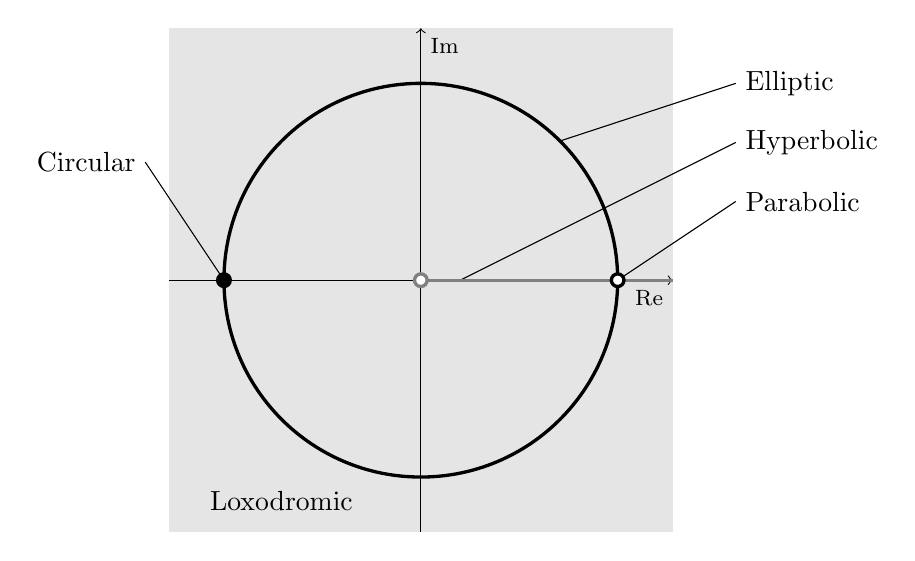
\begin{tikzpicture}

    \fill[gray!20] (-3.2, -3.2) rectangle (3.2, 3.2);

    \draw[very thick] (0, 0) circle (2.5 cm); 
    \draw[->] (-3.2, 0) -- (3.2, 0) node[anchor=north east] {\footnotesize{Re}};
    \draw[->] (0, -3.2) -- (0, 3.2) node[anchor=north west] {\footnotesize{Im}};

    \draw (0.5, 0) -- (4, 1.75) node[anchor=west] {Hyperbolic};
    \draw (2.5, 0) -- (4, 1) node[anchor=west] {Parabolic};
    \draw[gray, very thick] (0, 0) -- (3.2, 0);

    \filldraw[fill=white, very thick] (2.5, 0) circle (0.08 cm);
    \filldraw[fill=black, very thick] (-2.5, 0) circle (0.08 cm);
    \filldraw[color=gray, fill=white, very thick] (0, 0) circle (0.08 cm);

    \node[anchor=west] at (-2.8, -2.8) {Loxodromic};
    \draw (1.7677669529663689, 1.7677669529663689) -- (4, 2.5) node[anchor=west] {Elliptic};

    \draw (-2.5, 0) -- (-3.5, 1.5) node[anchor=east] {Circular};

    \node[anchor=south east] at (3.2, -3.2) {\(\complex\)};

\end{tikzpicture}
 
    \caption{Classification of Möbius transform in terms of the location of the multiplier \(k\) in the complex plane. Any point that is not on the unit circle yields a loxodromic transform; a particular subclass are the hyperbolic transforms, which are on the real axis except at \(-1\) and \(1\) where it intersects with the unit circle, and at the origin, where the transform becomes singular. If the multiplier lies on the unit circle except 1 are elliptic transforms, a special case is the circular transform for \(k = -1\). Finally, the parabolic transforms have a multiplier of 1 \cite{Needham1997}.}
    \label{fig:multiplier_regions}
\end{figure}
To summarize, there are five different classes of Möbius transform: circular, elliptic, hyperbolic, loxodromic and parabolic. Circular transforms are part of the elliptic transforms and hyperbolic transforms are a subclass of loxodromic transforms. The class to which a Möbius transform belongs is determined completely by its trace \(a + d\), or equivalently, the value of the multiplier \(k\). For the multiplier, one can distinguish several `regions' in the complex plane that are each associated with a class of Möbius transforms, this is visualized in \cref{fig:multiplier_regions}. The nature of the Jordan form of the matrix associated to a Möbius transform also clearly give away to which class a transform belongs. 
\begin{figure}
    \centering
    \begin{tikzpicture}
    \node at (0, 0) {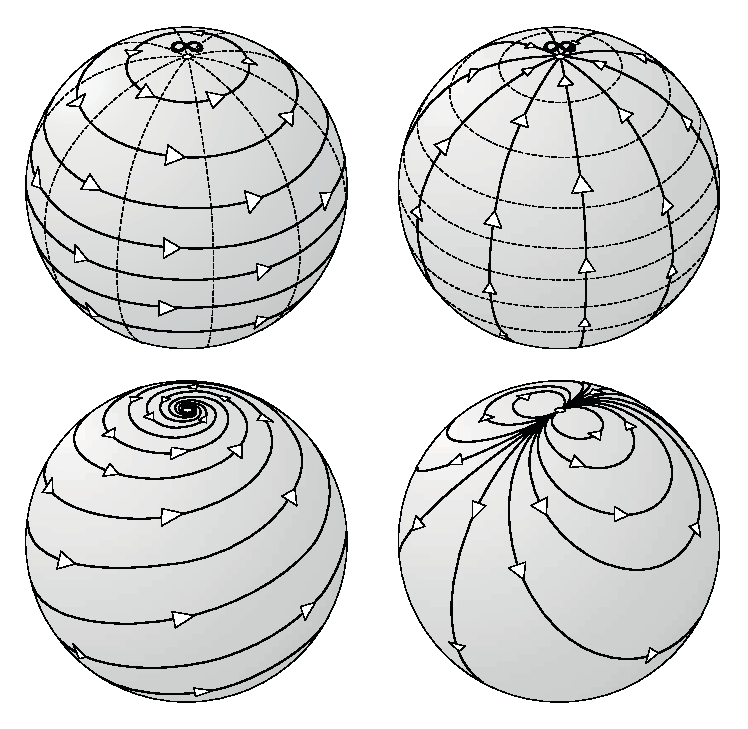
\includegraphics{media/tikz/mobius_transforms_needham.eps}};
    \node at (-3.1, 6.3) {\textbf{Elliptic}};
    \node at (3.2, 6.3) {\textbf{Hyperbolic}};
    \node at (-3.3, -6.3) {\textbf{Loxodromic}};
    \node at (3.3, -6.3) {\textbf{Parabolic}};
    \draw (-6.5, 0) -- (6.5, 0);
    \draw (0, -6.5) -- (0, 6.5);
\end{tikzpicture}

    \caption{Overview of the four classes of Möbius transform and their typical action on the Riemann sphere. The curves shown on the Riemann sphere are the \emph{invariant curves} of the transformation, i.e. these curves as a whole remain invariant under the transformation. Clearly, the elliptic, hyperbolic and loxodromic transformations have the North and South pole, or \(\infty\) and 0 as fixed points, whereas the parabolic transformation only has a single fixed point at the North pole. The loxodromic transformations borrow their name from loxodromes, which are spiral-like trajectories on the Earth with constant bearing --- a ship that taking a loxodromic path would maintain a constant angle with respect to true North. Illustration reprinted from \citet[p. 78]{Needham2021}.}
    \label{fig:riemann_transforms}
\end{figure}

\Cref{tab:moebiusclasses} provides an overview of the five Möbius classes, together with the values for the matrix trace, the multiplier and the Jordan form. Finally, \cref{fig:riemann_transforms} visualizes the effect of each of the transform classes on points on the Riemann sphere. Elliptic transforms push points along circles of constant latitude, while hyperbolic transforms move points orthogonally, along the meridians of the Riemann sphere. %Loxodromic transforms are compositions of hyperbolic and elliptic transforms, the associated trajectories therefore look like spirals; incorporating both a North-South and an East-West movement.
\begin{table}
    \caption{Overview of the five classes of Möbius transforms and the corresponding values for the trace squared of the matrix (\(\trace{M} = a + d\)), the multiplier of the transform and the Jordan form.}
    \label{tab:moebiusclasses}
    \centering
    \begin{tabular}{lcccc}
        \toprule
        \textbf{Class} & \textbf{Multiplier} & 
        \(\qty(a + d)^2\) & \textbf{Jordan form} & \textbf{Parent class} \\
        \midrule
        Circular    & \(\qty{-1}\)  &  \([0, 4)\) & 
                      \(\mqty(0 & -1 \\ 1 & 0)\) & Elliptic   \\[0.8cm]
        Elliptic    & \(\qty{k \in \complex \mid \abs{k} = 1, k \neq 1}\)   &  \([0, 4)\) &
                      \(\mqty(\ec^{\theta\ii/2} & 0 \\ 0 & \ec^{-\theta\ii/2})\) & ---  \\[0.8cm]
        Parabolic   & \(\{1\}\)  &  \(\qty{4}\)  & 
                      \(\mqty(1 & b \\ 0 & 1)\) & --- \\[0.8cm]
        Hyperbolic  & \(\real^+_{0} \setminus \qty{1}\) & \((4, +\infty)\)& 
                      \(\mqty(\ec^{\zeta/2} & 0 \\ 0 & \ec^{-\zeta/2})\) & Loxodromic \\[0.8cm]
        Loxodromic  & \(\qty{k \in \complex \mid \abs{k} \neq 1 }\)  & \(\complex\setminus[0, 4]\) &
                      \(\mqty(k & 0 \\ 0 & k^{-1})\) & --- \\[0.4cm]
        \bottomrule
    \end{tabular}
\end{table}

\section{Subgroups}
Apart from the classification considered in the preceding chapter, there are also several subgroups of the Möbius group that can be distinguished. It is compelling to observe that each of these subgroups can each be identified with one of the `geometry types' that were considered in \cref{chap:hyperbolic_geometry}: those of positive (spherical), zero (Euclidean) and negative (hyperbolic) geometry. For every geometry type, a specific subgroup of the Möbius group will play the role of the direct isometry group in a particular `map' \cite{Needham2021}.

\subsection{Euclidean geometry}
The direct isometries in the Euclidean plane consist simply of translations and rotations. Clearly, a rotation in the complex plane (around the origin) can be represented simply by \(z \mapsto e^{\ii \theta}\), while a translation is \(z \mapsto z + b\) with \(b \in \complex\). Hence, the entire direct isometry group of the Euclidean plane is given by
    \[ \mathfrak{E}(z) = e^{\ii\theta} + b. \]
This group is also called the Euclidean group of dimension two.
\subsection{Spherical geometry}
One of the most prevalent applications of group theory is are the representation of rotations in three-dimensional Euclidean space. Of course, the group associated with these rotations is the special orthogonal group \(\sogroup\). This group is diffeomorphic to the three-dimensional real projective space \(\mathbb{RP}^3\) (intuitively, this space consists of three `directions'). The rotations in \(\real^3\) can also be parameterized by \emph{unit quaternions} (also called \emph{versors}): these represent points on the 3-sphere \(\sphere{3}\). The difference between the 3-sphere and the real projective space is that the latter identifies the \emph{antipodal} parts that are present on the sphere. As such, any rotation in \(\real^3\) corresponds precisely to two points on the 3-sphere (or two unit quaternions) --- the group of unit quaternions therefore is a double cover of \sogroup. 

Quaternions can also be represented as complex matrices: \cite{Stillwell2008}
\[ q = \quat{m}{n}{o}{p} \in \quaternions \corresponds Q = \mqty(m + \ii p & -n - \ii o\\n - \ii o & m - \ii p),\]
which is a general represention of a \(2\times 2\) \emph{unitary}\footnote{A unitary matrix is a matrix whose inverse is its conjugate transpose --- it is the complex counterpart of orthogonal matrices.} matrix. Likewise, the unit quaternions then translate to matrices of the above type with an additional restriction: they must have a determinant of 1: these matrices are members of the \emph{special unitary group} \sugroup{2}. As such, the group of unit quaternions is isomorphic to the \sugroup{2} which is therefore also a double cover of \sogroup.

Since the members of \sugroup{2} can be identified with a Möbius transform (inspection of the matrix above makes this immediately apparent), a specific subgroup of \moebiusgroup can be used to represent the rotations in \(\real^3\) --- recall that every normalized Möbius transform also corresponds to two matrices, differing by a factor -1. Observing the matrix above, one can see that the entries on the main diagonal are each others' conjugate, while the entries on the antidiagonal are conjugate opposite. Therefore, the general expression of a rotation of the Riemann sphere as a Möbius transform can be written as: \cite{Needham2021}
\[\mathfrak{S} = \frac{az + b}{-\conj{b}z+\conj{a}}\quad\text{where } \abs{a}^2 + \abs{b}^2 = 1; \]
the latter equivalent then enforces that \(\det Q = 1\). There are always two quaternions representing the same rotation; they are antipodal and differ by a factor of \(-1\). As a result, there are two possibilities for \(Q\) as well, again identical but with opposite entries. Recall that the same applies to the matrix representations of Möbius transforms: as such, the ambiguities are eliminated, and the group of transforms of type \(\mathfrak{S}\) is isomorphic to \sogroup. In the complex plane, these transformations represent the isometries of spherical geometry in the stereographic map \cite{Needham1997}. 

\index{versor}
\index{quaternion}

\subsection{Hyperbolic geometry}
As described by \citet{Rovenski2010}, the isometries of the Poincaré half-plane are any (composition) of the following types of transformations, i.e. they leave distances according to the Poincaré metric unaffected:
\begin{itemize}
    \item horizontal translations: \((x, y)\mapsto(x + a, y)\) where \(x, y, a \in real\);
    \item reflection around the vertical axis: \((x, y) \mapsto (-x, y)\);
    \item dilations centered around the origin: \((x, y) \mapsto (ax, ay)\);
    \item inversions with respect to the unit circle \((x, y)\mapsto\qty(\frac{x}{x^2 + y^2}, \frac{y}{x^2 + y^2})\).
\end{itemize}
The group of all these transformations is precisely \pslgroup{2}{\real}, or the Möbius tranforms with real parameters:
\[\mathfrak{H}(z) = \frac{az + b}{cz + d}\qquad a, b, c, d \in \real \quad ad - bc = 1;\]
these are the isometries of the Poincaré half plane \cite{Needham2021}. Recall from \cref{ssec:poincare_halfplane} that there are two types of geodesics in the half plane: semicircles centered at the origin and straight (from Euclidean perspective) vertical lines. These are precisely invariant curves for the transformations listed --- isometries take geodesics to geodesics \cite{Lee1997}.

\section{Relation with other groups}
Another classic Lie group is the special linear group \slgroup{n}{\field}, which are the volume-preserving transformations on a vector space --- this property turns out to be quite important. The special linear group over the complex numbers (2-dimensional) \slgroup{2}{\complex} can be represented as the group of all the complex \(2\times2\) matrices with unit determinant. It has been mentioned previously that any such matrix coincides with a Möbius transform, albeit surjectively: for every Möbius transform, there are two such matrices. As such, \slgroup{2}{\complex} is a \emph{double cover} of \moebiusgroup.

Arguably more interesting than \slgroup{2}{\complex} is the special linear group over the reals \slgroup{2}{\real}, i.e. every invertible \(2 \times 2\) matrix with real entries and a unit determinant; they form a subgroup of \slgroup{2}{\complex} as well. It has been mentioned before that the for the normalized Möbius transforms, the eigenvalues should be complex inverses of each other. For matrices with real entries, the eigenvalues are either both real or complex conjugates of each other. When not on the real axis, the only way eigenvalues can be complex inverses and complex conjugate is to be located on the unit circle. As can be seen on \cref{fig:multiplier_regions}, that means that the matrices with real entries contain exactly the hyperbolic (both real), elliptic (unit circle) and parabolic classes. The remaining part are the loxodromic transforms which have a nonreal trace.

\towrite{TODO}

\begin{figure}
    \centering
    \begin{tikzpicture}
    \node[draw, align=center, thick] (moebius) at (0, 0) {\scriptsize{Möbius group}\\\moebiusgroup = \automorphgroup{\hat{\complex}}};
    \node[draw, align=center] (lorentz) at (0, -2) {\scriptsize{Lorentz group}\\\restlorentzgroup};
    \node[draw, align=center] (psl) at (4, 0) {\scriptsize{Projective special linear group}\\\pslgroup{2}{\complex}};
    \node[draw, align=center] (pgl) at (4, -2) {\scriptsize{Projective linear group}\\\pglgroup{2}{\complex}};

    \node[draw, align=center] (slc) at (0, 4) {\slgroup{2}{\complex}};
    \node[draw, align=center] (slr) at (4, 4) {\slgroup{2}{\real}};

    \node[draw, align=center] (e) at (-4, -2) {\(\mathfrak{E}\)};
    \node[draw, align=center] (s) at (-4, 0) {\(\mathfrak{S}\)};
    \node[draw, align=center] (h) at (3, 1.5) {\(\mathfrak{H}\)};

    \node[draw, align=center] (euclidean) at (-4, -4) {\scriptsize{Euclidean group}};
    \node[draw, align=center] (su) at (-4, 5) {\scriptsize{Special unitary group}\\\sugroup{2}};
    \node[draw, align=center] (so) at (-4, 2) {\scriptsize{Special orthogonal group}\\\sogroup};

    \node[draw, align=center] (su11) at (5, 6) {\scriptsize{Special unitary group}\\\sugroup{1, 1}};
    \node[draw, align=center] (sp) at (1, 6) {\scriptsize{Symplectic group}\\\spgroup{2}{\real}};
    
    \draw[style=double] (moebius) -- (lorentz);
    \draw[style=double] (moebius) -- (psl);
    \draw[style=double] (lorentz) -- (psl);
    \draw[style=double] (lorentz) -- (pgl);
    \draw[style=double] (moebius) -- (pgl);
    \draw[style=double] (pgl) -- (psl);
    \draw[style=double] (s) -- (so);
    \draw[style=double] (e) -- (euclidean);
    \draw[style=double] (su11) -- (sp);
    \draw[style=double] (slr) -- (sp);
    \draw[style=double] (slr) -- (su11);

    \draw[->] (slc) -- (moebius) node[pos=0.5, sloped, anchor=centre, above] {\scriptsize{double cover}};
    \draw[->] (slr) -- (slc) node[pos=0.5, sloped, anchor=centre, above] {\scriptsize{subgroup}};
    \draw[->] (e) -- (moebius) node[pos=0.5, sloped, anchor=centre, above] {\scriptsize{subgroup}};
    \draw[->] (s) -- (moebius) node[pos=0.5, sloped, anchor=centre, above] {\scriptsize{subgroup}};
    \draw[->] (h) -- (moebius) node[pos=0.5, sloped, anchor=centre, above] {\scriptsize{subgroup}};
    \draw[->] (su) -- (so) node[pos=0.5, sloped, anchor=centre, above] {\scriptsize{double cover}};
    \draw[->] (slr) -- (h) node[pos=0.5, sloped, anchor=centre, above] {\scriptsize{double cover}};
\end{tikzpicture}

    \caption{Schematic of the relation of the Möbius group with other important groups such as the special orthogonal group, special unitary group, Lorentz group etc.}
\end{figure}

